\documentclass{article}

\usepackage{xcolor}
\setlength{\parindent}{0pt}

\usepackage{listings}
\lstset{basicstyle=\ttfamily}
\renewcommand{\lstlistlistingname}{Índice de programas}
\renewcommand{\lstlistingname}{Programa}

%\usepackage{listingsutf8}
%\lstset{inputencoding=utf8/latin1}

\usepackage{tikz}
\newcommand*{\tikzgrid}[2]{\draw[help lines](0,0)grid[step=0.2,lightgray,ultra thin](#1,#2);\draw[help lines](0,0)grid[gray](#1,#2);\foreach\x in{0,1,...,#1}\node[below]at(\x,0){\scriptsize\x};\foreach\y in{1,2,...,#2}\node[left]at(0,\y){\scriptsize\y};} 
\usetikzlibrary{arrows.meta}

\begin{document}
	
\begin{figure}	
	\centering
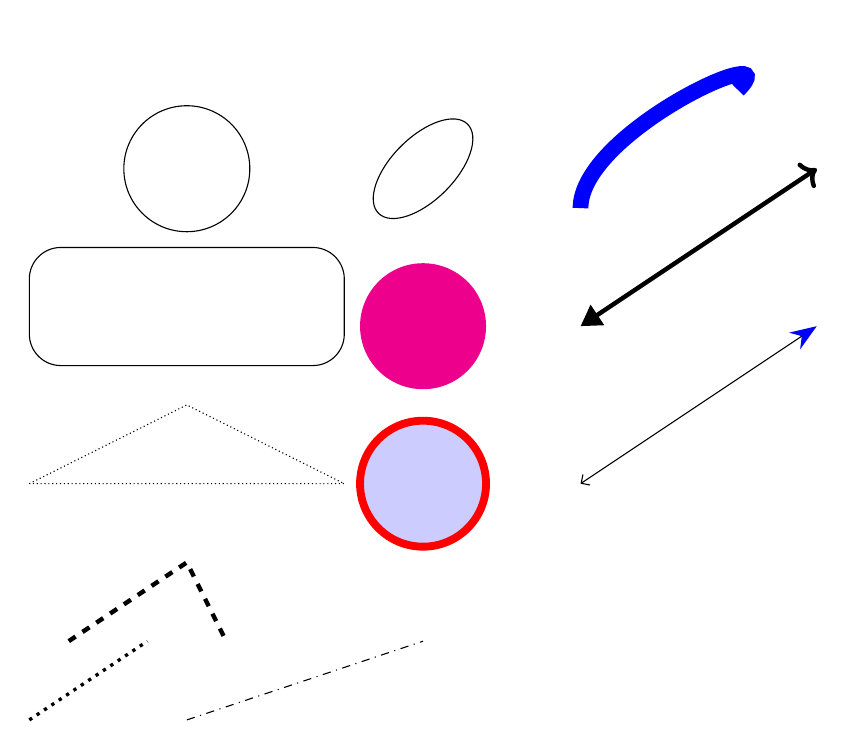
\begin{tikzpicture}
%\tikzgrid{12}{8}
\path[draw,ultra thick,dashed](0.5,1)--(2,2)--(2.5,1);
\draw[very thick,dotted](0,0)--(1.5,1);
\draw[densely dotted](0,3)--(2,4)--(4,3)--cycle;
\draw[rounded corners=4mm](0,4.5)rectangle(4,6);
\draw(2,7)circle[radius=0.8cm];
\draw(5,7)circle[x radius=8mm,y radius=4mm,rotate=45];
\draw[blue,line width=2mm](7,6.5)to[out=90,in=45](9,8);
\fill[magenta](5,5)circle[radius=8mm];
\filldraw[draw=red,fill=blue!20, line width=1mm](5,3)circle[radius=8mm];
\draw[dash dot](2,0)--(5,1);

\draw[arrows=Triangle->,ultra thick](7,5)--(10,7);
\draw[arrows={Straight Barb-Stealth[scale=2,blue]}](7,3)--(10,5);
\end{tikzpicture}
\caption{mi primer gráfico usando tikz}
\end{figure}	

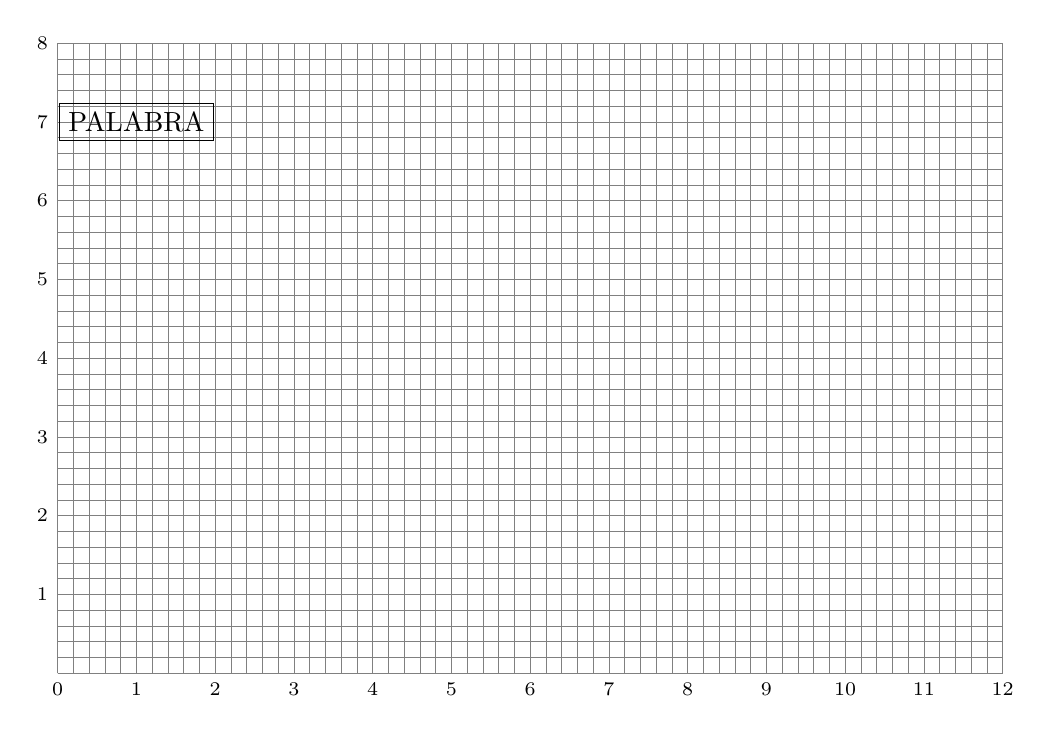
\begin{tikzpicture}
\tikzgrid{12}{8}
\node[draw]at(1,7){PALABRA};
\end{tikzpicture}
	
	
	
	
	
	
	
	
	
	
	
	
	
	
	
	
	
	
	
	
	
\clearpage
	
\lstlistoflistings

\'a \'e \'i \'o \'u \~n

\begin{lstlisting}[mathescape=true,escapechar=|, inputencoding=utf8,literate={é}{{\'e}}1{ñ}{{\~n}}1]
$\int f(x)dx$ |texto normal mecánica|

// comentario en español té
#include <stdio.h>
int main()
{
int firstNumber, secondNumber, sumOfTwoNumbers;

printf("Enter two integers: ");

// Two integers entered by user is stored using scanf() function
scanf("%d %d", &firstNumber, &secondNumber);

// sum of two numbers in stored in variable sumOfTwoNumbers
sumOfTwoNumbers = firstNumber + secondNumber;

// Displays sum      
printf("%d + %d = %d", firstNumber, secondNumber, sumOfTwoNumbers);

return 0;
}
\end{lstlisting}
	
\begin{lstlisting}[caption={este es mi primer programa},captionpos=b,breaklines=true,frame=single,rulecolor=\color{red},backgroundcolor=\color{pink!30},frameround=tf]
#include <stdio.h>
int main()
{
int firstNumber, secondNumber, sumOfTwoNumbers;

printf("Enter two integers: ");

// Two integers entered by user is stored using scanf() function
scanf("%d %d", &firstNumber, &secondNumber);

// sum of two numbers in stored in variable sumOfTwoNumbers
sumOfTwoNumbers = firstNumber + secondNumber;

// Displays sum      
printf("%d + %d = %d", firstNumber, secondNumber, sumOfTwoNumbers);

return 0;
}
\end{lstlisting}
	
\begin{lstlisting}[language=C,basicstyle=\ttfamily\small\color{blue},showtabs=true,showspaces=true, numbers=left,numberstyle={\footnotesize\color{blue!30}},numberblanklines=false,firstnumber=90,caption={este es mi segundo programa}]
#include <stdio.h>
int main()
{
int firstNumber, secondNumber, sumOfTwoNumbers;

printf("Enter two integers: ");

// Two integers entered by user is stored using scanf() function
scanf("%d %d", &firstNumber, &secondNumber);

// sum of two numbers in stored in variable sumOfTwoNumbers
sumOfTwoNumbers = firstNumber + secondNumber;

// Displays sum      
printf("%d + %d = %d", firstNumber, secondNumber, sumOfTwoNumbers);

return 0;
}
\end{lstlisting}
	
\begin{lstlisting}[gobble=2]
#include <stdio.h>
  int main()
  {
  int firstNumber, secondNumber, sumOfTwoNumbers;

  printf("Enter two integers: ");

  // Two integers entered by user is stored using scanf() function
  scanf("%d %d", &firstNumber, &secondNumber);

  // sum of two numbers in stored in variable sumOfTwoNumbers
  sumOfTwoNumbers = firstNumber + secondNumber;

  // Displays sum      
  printf("%d + %d = %d", firstNumber, secondNumber, sumOfTwoNumbers);

  return 0;
  }
\end{lstlisting}
	
\newpage
	
texto texto texto \lstinline|\usepackage| texto texto 

\rule{7cm}{5mm}

\begin{lstlisting}[float=t,belowskip=3cm]
#include <stdio.h>
int main()
{
int firstNumber, secondNumber, sumOfTwoNumbers;

printf("Enter two integers: ");

// Two integers entered by user is stored using scanf() function
scanf("%d %d", &firstNumber, &secondNumber);

// sum of two numbers in stored in variable sumOfTwoNumbers
sumOfTwoNumbers = firstNumber + secondNumber;

// Displays sum      
printf("%d + %d = %d", firstNumber, secondNumber, sumOfTwoNumbers);

return 0;
}
\end{lstlisting}



\lstinputlisting[firstline=8,lastline=25]{picins.sty}
\lstinputlisting[linerange={8-25}]{picins.sty}

\lstinputlisting[language=TeX,breaklines=true]{picins.sty}


%\lstinputlisting{picins2.sty}
	
\newpage	

\begin{verbatim}
#include <stdio.h>
int main()
{
	int firstNumber, secondNumber, sumOfTwoNumbers;
	
	printf("Enter two integers: ");
	
	// Two integers entered by user is stored using scanf() function
	scanf("%d %d", &firstNumber, &secondNumber);
	
	// sum of two numbers in stored in variable sumOfTwoNumbers
	sumOfTwoNumbers = firstNumber + secondNumber;
	
	// Displays sum      
	printf("%d + %d = %d", firstNumber, secondNumber, sumOfTwoNumbers);
	
	return 0;
}	
\end{verbatim}	

\end{document}